\section{Introduzione}
Sempre più giochi da tavolo ormai vantano una versione digitale,
caratterizzata dalla possibilità di permettere agli utenti di giocare in
modalità multiplayer.
Allo stesso tempo però sono ancora rare implementazioni distribuite di
giochi multiplayer le quali spesso sono invece basate su un architettura
client server. In questo documento descriveremo il nostro lavoro di
progettazione ed implementazione della versione software di un gioco da
tavolo con particolare interesse riguardo l'architettura di rete
distribuita utilizzata nella modalità multiplayer.

\subsection{Carcassone}
In particolare è stato nostro interesse occuparci del remake del gioco
da tavolo Carcassonne. Quest'ultimo nello specifico è un boardgame dei
primi anni 2000 basato su tessere che consiste nel creare un paesaggio medievale 
posizionando e accostando tra loro vari tipi di tessere, che rappresentano una parte di città, 
un tratto di strada, un campo o un monastero \footnote{Si fa riferimento
alla prima versione del gioco in cui non sono presenti fiumi}.
Completando quindi più città, strade, ecc, attraverso tali tessere, i
giocatori (previsti da 2 a 5) accumulano i punti necessari a vincere la partita.
Al fine di comprendere al meglio le prossime sezione di questo documento, 
vedremo
brevemente di seguito il funzionamento del gioco.
All'inizio della partita, una singola tessera è posizionata sul tavolo, scoperta; 
le altre tessere sono posizionate coperte nel mazzo e mischiate.
Ciascuna di tali tessere rappresenta un frammento di paesaggio, e può contenere uno o più dei seguenti elementi:

\begin{itemize}
	\item tratti di strada, inclusi incroci e curve
    \item aree cittadine racchiuse da mura
    \item campi che circondano le città e accolgono le strade
    \item un monastero
\end{itemize}


\begin{figure}[H]
\centering
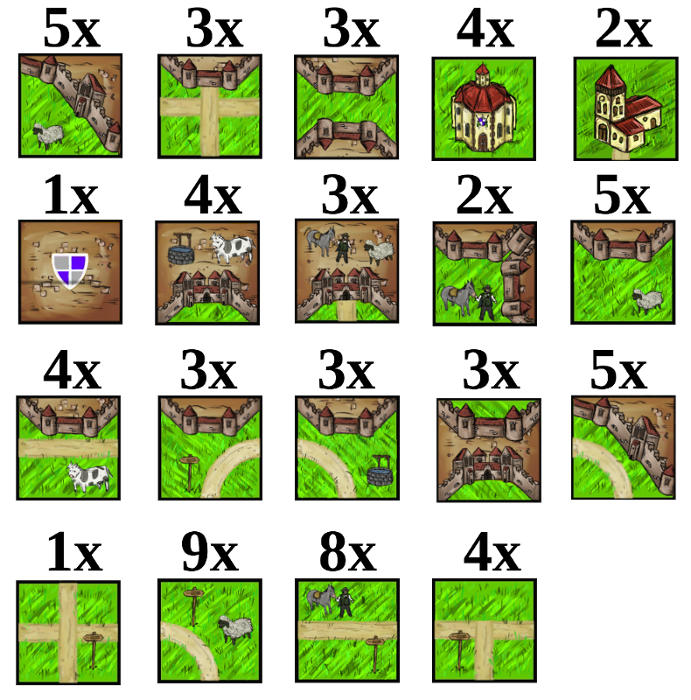
\includegraphics[scale=0.4]{img/tiles.png}
\caption{Elenco delle tessere presenti nel gioco}
\label{img:tiles}
\end{figure}

A turno, i giocatori estraggono una tessera dal mazzo e la posizionano scoperta sul tavolo
in contatto con le tessere già piazzate attraverso uno o più lati in modo coerente con le altre, 
in modo da proseguire eventuali strade, campi, o mura già presenti.

Dopo aver posizionato la tessera, il giocatore può decidere di piazzare
una pedina detta \emph{meeple} su di essa che reclama la proprietà di un elemento di terreno
 e non può essere piazzato su un elemento già reclamato da un altro
meeple. Può accadere comunque che un elemento possegga più di un
proprietario se diviene una congiunzione di due elementi dello stesso
tipo non precedentemente adiacenti.
Quando un elemento viene completato, se ad esempio le mura di una città

vengono chiuse o se una strada ha due estremità chiuse, il proprietario
di quell'elemento acquisisce i relativi punti. Il punteggio di un
elemento è dipendente dal numero e dal tipo di tessere che compongono
l'elemento.

Il gioco termina con il piazzamento dell'ultima tessera; vince il giocatore che ha totalizzato più punti.

Rimandiamo alla documentazione ufficiale di Carcassonne per ulteriori
dettagli.

La semplice struttura del gioco e la sua organizzazione a turni rende
interessante l'approccio distribuito in quanto si evita di incorrere in problemi 
di prestazioni tipici dei giochi reattivi. Quest'ultimi infatti hanno requisiti prestazionali molto stringenti. In
particolare spesso richiedono che le comunicazioni di rete siano a bassa
latenza al fine di impedire il più possibile agli utenti di giocare con
artefatti grafici fastidiosi dovuti ai ritardi di rete o all'overhead di
comunicazione.\\
Come già accennato, il gioco da noi considerato necessita invece di
requisiti prestazionali più laschi soprattuto per i lunghi tempi
decisionali degli utenti (comparati ai tempi di rete e computazionali).
\\
Vedremo nelle prossime sezioni i dettagli progettuali ed implementativi.
In ultimo forniremo una analisi valutativa dei risultati ottenuti dai test
con le dovute considerazioni finali.
